\section{Statistical analysis}
In the last chapter, the agreement between MC and data was qualitatively inspected.
To judge the agreement between data and the background-only hypothesis, a $\chi^2$ test will be performed using MC simulations as the background-only hypothesis.
The value of $\chi^2$ is a metric for the deviation of the data and MC sample.
If the background-only hypothesis  and data are in a good agreement, meaning no $Z^\prime$ exists, $\chi^2$ will have a small value.
In this case an exclusion limit will be set on the production cross section.
For that a confidence level is needed that is calculated with
\begin{equation}
  \text{CL}= 1-p
\end{equation}
with $p$ as the $p$-value for the background-only hypothesis.

The results of the $\chi^2$ test are:
\begin{align*}
  \chi^2= 25.1862 \\
  p = 0.508458
\end{align*}
Even though a high $\chi^2$ value is achieved, the $p$-value is very high as well.
This shows that the found peaks in the invariant mass is just a statistical fluctuation and that no observation of a $Z^\prime$ is found.
Therefore an exclusion limit for the different $Z^\prime$ mass hypotheses will be calculated in a $\SI{95}{\percent}$ confidence level.
To consider the weights, a scaler will be used that scales the weights until the confidence level is reached.
These results are shown in table \ref{tab:chi2}.

\begin{table}
  \centering
  \caption{Calculated parameters of the $\chi^2$ test for the different  $Z^\prime$ mass hypothises as well as the cross section exclusion limit in a  $\SI{95}{\percent}$ confidence level.}
  \label{tab:chi2}
  \begin{tabular}{c|cccc}
    \toprule
    process & degrees of freedom & $p$-value & scaler & $\sigma / \si{\pico b}$ \\
    $Z^\prime (400)$  & 26 & 0.00549806 & 0.4 & 44 \\
    $Z^\prime (500)$  & 26 & 0.00211708 & 0.2 & 16.4 \\
    $Z^\prime (750)$  & 26 & 0.0150853  & 0.2 & 4 \\
    $Z^\prime (1000)$ & 26 & 0.0472768 & 0.4 & 2.2 \\
    $Z^\prime (1250)$ & 26 & 0.0394068 & 0.9 & 1.71 \\
    $Z^\prime (1500)$ & 26 & 0.0433432 & 1.9 & 1.58 \\
    $Z^\prime (1750)$ & 26 & 0.0462103 & 4.8 & 1.44 \\
    $Z^\prime (2000)$ & 26 & 0.0499252 & 10.9 & 1.526 \\
    $Z^\prime (2250)$ & 26 & 0.0495314 & 23.5 & 1.57 \\
    $Z^\prime (2500)$ & 26 & 0.0498703 & 48.7 & 1.70 \\
    $Z^\prime (3000)$ & 26 & 0.0499869  & 194.7 & 2.33 \\
    \midrule
    \bottomrule
  \end{tabular}
\end{table}

The resulting cross section at the $\SI{95}{\percent}$ confidence level are being compared against the expected cross sections in figure \ref{fig:limit}.
Since the observed cross section is smaller than theoretically predicted, masses of $m_{Z^\prime} \textless \SI{1300}{\giga\electronvolt}$ can be excluded.
A particle with a lower mass would have been observed in this analysis.
Masses of $m_{Z^\prime} \textgreater \SI{1300}{\giga\electronvolt}$ could not be discriminated from the background so that these masses are not excluded in this analysis.

\begin{figure}
    \centering
    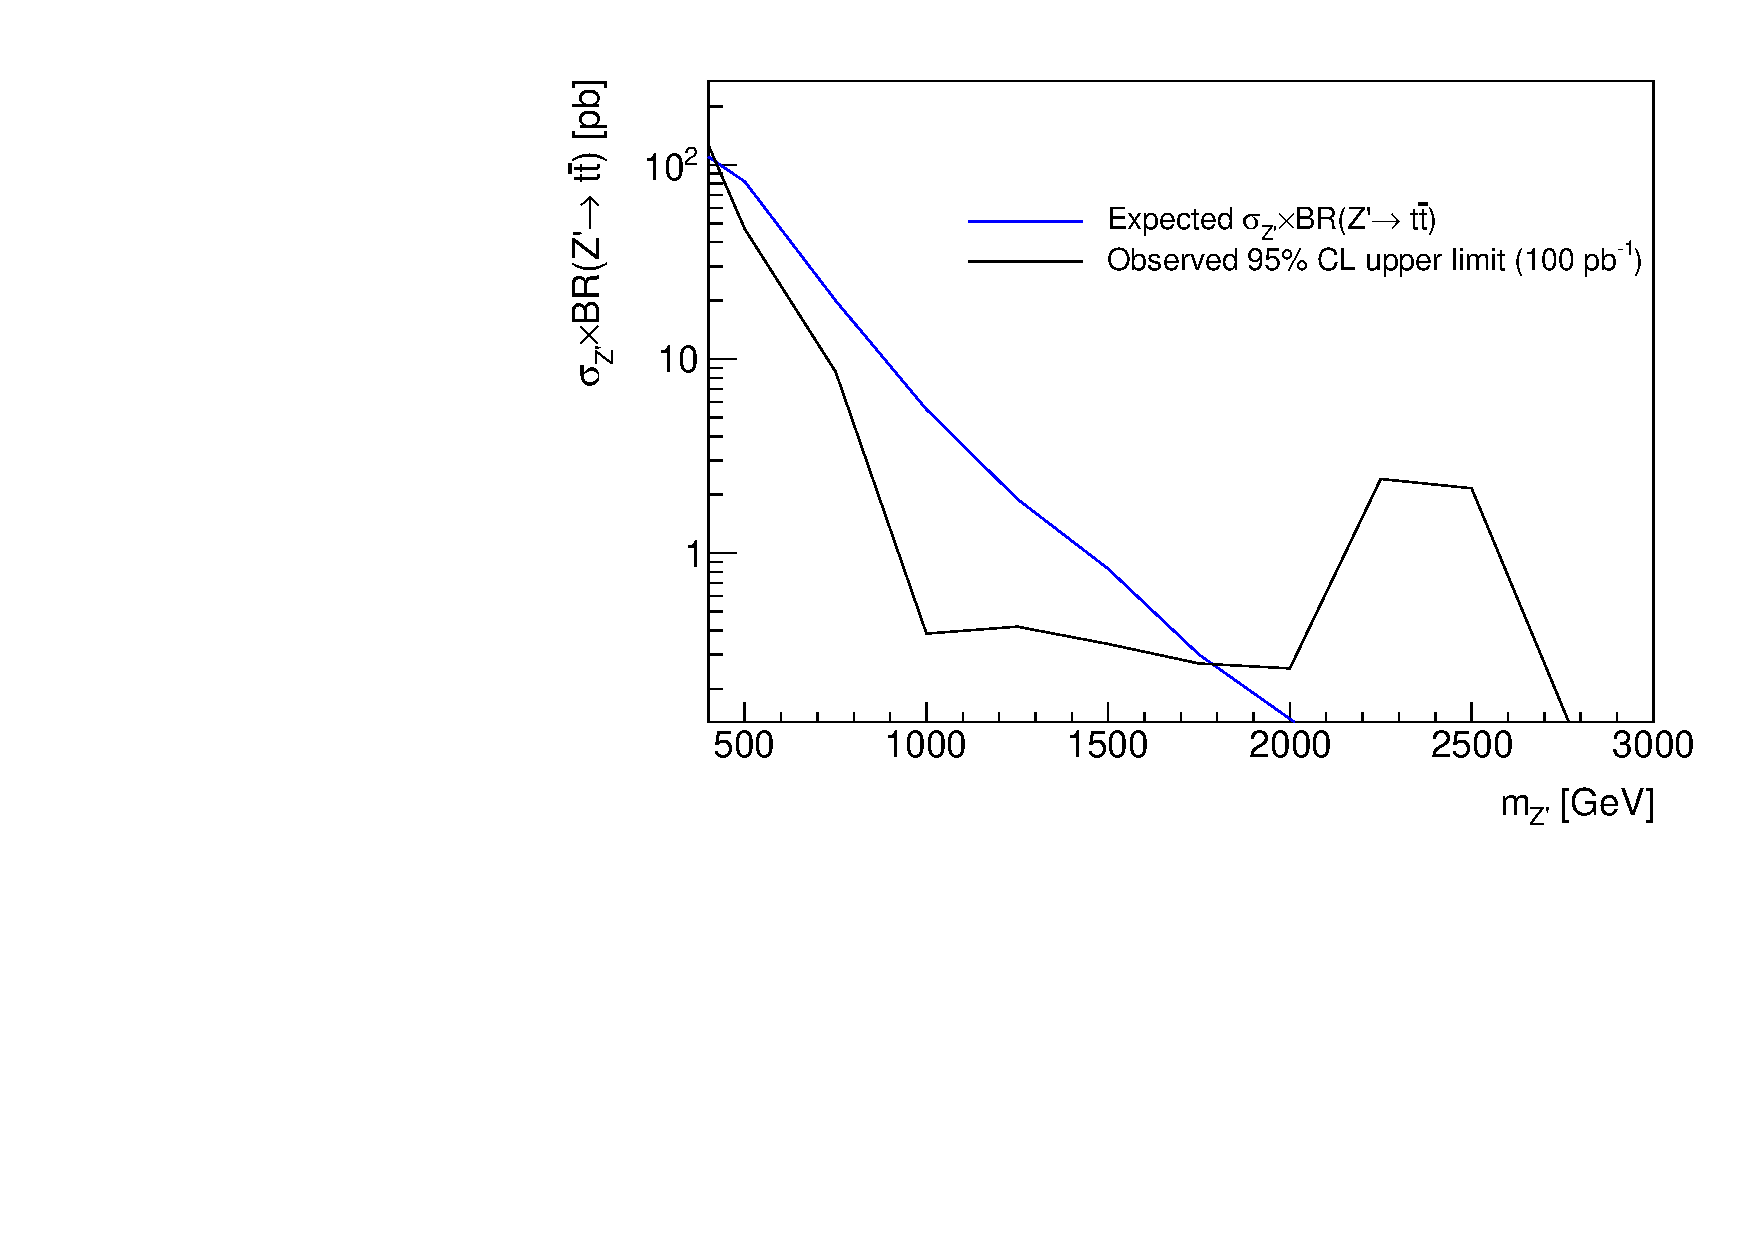
\includegraphics[width=\linewidth]{plots/limits.pdf}
    \caption{Calculated upper limits of the cross section in a $\SI{95}{\percent}$ confidence level for the different $Z^\prime$ mass hypothises. For comparison, the expected cross section is plotted as well.}
    \label{fig:limit}
\end{figure}
